% THIS IS SIGPROC-SP.TEX - VERSION 3.1
% WORKS WITH V3.2SP OF ACM_PROC_ARTICLE-SP.CLS
% APRIL 2009
%
% It is an example file showing how to use the 'acm_proc_article-sp.cls' V3.2SP
% LaTeX2e document class file for Conference Proceedings submissions.
% ----------------------------------------------------------------------------------------------------------------
% This .tex file (and associated .cls V3.2SP) *DOES NOT* produce:
%       1) The Permission Statement
%       2) The Conference (location) Info information
%       3) The Copyright Line with ACM data
%       4) Page numbering
% ---------------------------------------------------------------------------------------------------------------
% It is an example which *does* use the .bib file (from which the .bbl file
% is produced).
% REMEMBER HOWEVER: After having produced the .bbl file,
% and prior to final submission,
% you need to 'insert'  your .bbl file into your source .tex file so as to provide
% ONE 'self-contained' source file.
%
% Questions regarding SIGS should be sent to
% Adrienne Griscti ---> griscti@acm.org
%
% Questions/suggestions regarding the guidelines, .tex and .cls files, etc. to
% Gerald Murray ---> murray@hq.acm.org
%
% For tracking purposes - this is V3.1SP - APRIL 2009
\documentclass{acm_proc_article-sp}

\usepackage[utf8]{inputenc}
\begin{document}

\title{Major Language Detection}
%
% You need the command \numberofauthors to handle the 'placement
% and alignment' of the authors beneath the title.
%
% For aesthetic reasons, we recommend 'three authors at a time'
% i.e. three 'name/affiliation blocks' be placed beneath the title.
%
% NOTE: You are NOT restricted in how many 'rows' of
% "name/affiliations" may appear. We just ask that you restrict
% the number of 'columns' to three.
%
% Because of the available 'opening page real-estate'
% we ask you to refrain from putting more than six authors
% (two rows with three columns) beneath the article title.
% More than six makes the first-page appear very cluttered indeed.
%
% Use the \alignauthor commands to handle the names
% and affiliations for an 'aesthetic maximum' of six authors.
% Add names, affiliations, addresses for
% the seventh etc. author(s) as the argument for the
% \additionalauthors command.
% These 'additional authors' will be output/set for you
% without further effort on your part as the last section in
% the body of your article BEFORE References or any Appendices.

\numberofauthors{1} %  in this sample file, there are a *total*
% of EIGHT authors. SIX appear on the 'first-page' (for formatting
% reasons) and the remaining two appear in the \additionalauthors section.
%
\author{
% You can go ahead and credit any number of authors here,
% e.g. one 'row of three' or two rows (consisting of one row of three
% and a second row of one, two or three).
%
% The command \alignauthor (no curly braces needed) should
% precede each author name, affiliation/snail-mail address and
% e-mail address. Additionally, tag each line of
% affiliation/address with \affaddr, and tag the
% e-mail address with \email.
%
\alignauthor
       Juraj Hreško, Vojtěch Diatka, Kryštof Bořkovec \\
       \affaddr{Seznam.cz, a.s.}\\
       \affaddr{Radlická 3294/10}\\
       \affaddr{Prague 5, Czech Republic}\\
       \email{\{juraj.hresko,vojtech.diatka,krystof.borkovec\}@firma.seznam.cz}
}

\maketitle
\begin{abstract}
TODO
\end{abstract}
\keywords{language detection, classification, LETOR} % NOT required for Proceedings

\section{Introduction}
  Delivering the content based on the preferences of the user is one of the basic tasks of information retrieval systems.
  The most important content parameter is called relevance. 
  However, this parameter contains somehow inherently other parameters one of which we could call usability.
  This hidden parameter could be defined as a probability that user will be able to use the content of particular 
  document to satisfy his (intended) needs.
  Usability of the document is not solely a parameter of a document. 
  We could say that it is a parameter of the user - document relation.

  Language of the document affects the usability with different intensity. 
  The weight of its influence depends on the type of document content.
  For example, there is almost no need for understanding the language of the page if it provides mainly images or video content.
  Document readability is telling us if particular user is able to
  "use" texts on the web page for his intent (e.g. reading a joke, comments or navigation elements).
  
  The readability could be easily measured if we know that the page contains texts written in only one language 
  and if we know the languages known by the user.
  E.g. we can say that the document written solely in some language $L_a$ would not be readable for a reader 
  that does not know language $L_a$. 
  In this case (when there is only one language used on the page) 
  the so called "major" language of the page is $L_a$, further on denoted by $L_{maj} = L_a$.
  
  However, there are many documents that contains more than one language.
  Finding out languages and their proportion on a webpage is well-established topic in computational processing of web pages (citace).
  It could be harder to decide which language would be the "major" for these.
 
  Let us define the "major" language more precisely. 
  
  "Major" language ($L_{maj}$) of a given webpage is the intended language of all potential queries aiming at a given webpage.
  Intended language is the language of web pages in which a user intends to find results in SERP. 
  This definition implies that if a user searches for webpages in a language $L_a$, 
  our major goal is to provide webpages for which $L_{maj} = L_a$.
  
  For each webpage, we thus need to ask: “If the user wanted to find this page, in which language would he formulate the query?” 
  Our interpretation of major language presupposes that user knows what should be the language of the answer to his query.

  To choose the language $L_{maj}$ we used on-page language detection results and other features.
  We approached this topic with a machine-learning method based on our implementation of multiple additive oblivious decision trees called RC-rank.
  %It is essential topic for any full text search engine to return webpages relevant to a query. 
  %One of the dimensions of relevancy is also a language. 
  %This definition strives to exclude any ambiguity. There are very few contexts in which there would be more queries in various languages aiming at the same page.

\section{Related Work}

  To our knowledge, there is no paper dealing with choosing the main language from the set
  of languages identified on a webpage. Except for a few remarks on this topic in papers 
  focusing on on-page language detection this topic seems to be unexplored. 
  
  Necessary prerequisite for our research is on-page language detection. Many researchers approached this topic
  from various perspectives. For a comparison of some of these models, see \cite{Baldwin:shortlong}. 
  First algorithms were based on n-grams comparing frequencies of n-grams in a given document with 
  language models - frequency list of n-grams \cite{trenkle:ngram}. Current algorithms classifying languages 
  are based on Support Vector Machines (SVM). System based on SVM first maps input into a high dimensional space. 
  Then, it separates classes with a hyperplane (\cite{Campbell:supportvector}, \cite{Lodhi:textclass}).
  Our on-page identification was based on an algorithm by Řehůřek and Kolkus (\cite{Rehurek:languageidentification}).  They elaborated the n-gram approach. 
  “We propose and evaluate a new method, which constructs language models based on word relevance. We also 
  extend our method to allow us to efficiently and automatically segment the input text into blocks of individual 
  languages, in case of multiple-language documents.” (\cite{Rehurek:languageidentification})
  
  
  We would like to mention one example of how other researchers have dealt with our task. As it was not the main goal of 
  their paper, their solution is very simple:
  “In these cases, we try to re-apply the n-gram algorithm, weighting the largest continuous text block in the document 
  (blocks are identied in the HTML parsing stage, taking in account the markup information) as three times more important 
  than the normal text. The rationale for this is that the longest block will very likely correspond to a good description 
  of the page, possibly in its main language.” (\cite{Martins:langidentweb}) If we are to determine the major language of a website 
  we can’t confine ourselves to choose simply the language with highest proportion. A good example of this is a case of an online marketplace
  containing 80\% English and 20\% Czech. Despite this language proportion we would like to choose Czech as the main language. 
  English on this webpage comes up only as the names of products in a very long list. Only the navigational elements are labeled in Czech. In this case 
  we need to assign this page a Czech main language tag because we want to have it as a landing page for queries in Czech.

\section{Languages}

  For our purpose we needed to work with specific categories of languages.
  As a web fulltext search company we work with non-trivial volume of web documents.
  Due to technical limitations as well as because our services target mainly market in the Czech Republic,
  our database of indexed documents represents sample with specific language distribution (Table \ref{langdist}) which is different from the
  language distribution of all documents in the Internet.
  The distribution is based primarily on the list of "prefered" languages –
  Czech, English, Slovak, German, Polish and French –
  selected as most interesting latin-alphabet languages for local users and representing  our first six classes.
  As we are not trying to differentiate other languages, we created three other language classes specified only by writing system
  – latin, cyrillic and other (e.g. Hungarian, Bulgarian and Armenian language, respectively).

  \begin{table}[]
 \centering
 \caption{Languages distribution in dataset} 
 \label{langdist} 
 \vspace{0.5cm}
 \begin{tabular}{l||c}
    Czech & 61.9\% \\
    English & 19.1\% \\
    Slovak & 3.0\% \\
    German & 1.7\% \\
    Polish & 0.7\% \\
    French & 0.6\% \\ \hline
    Latin & 7.7\% \\
    Cyrillic & 3.2\% \\
    Other & 3.1\% \\
 \end{tabular}
 \end{table}


  \section{Classifier}

  Our task resembles a multi-class classification problem. 
  This approach brings a number of issues arising primarily from the fact of class multiplicity. 
  In the first place, there is a problem with sampling as we needed to keep corresponding proportions 
  of real distribution of languages across our dataset. 
  This leads to the situation when some classes examples are quite rare and so their count is insufficient 
  to train proper classifier. Also, this approach misses one generalisation valid for our data.
  We assume that all language classes behave uniformly with respect to feature values. In other words, 
  one combination of feature values based on presence of English leads to classifying the example as English whereas 
  the same or similar combination of feature values based on presence of Czech leads to classifying an example as Czech.
  In multi-category classification we lose this generalisation because all language-specific features are considered
  not to behave the same/similar way. If we want to capture this generalisation we can claim that feature values based on 
  presence of language $L_a$ leads to classifying an example as $L_a$. Therefore, we decided to approach our task as binary 
  classification problem. Apart from language specific features, such as proportion of English/Czech text on a given 
  web page, we included a \textit{generic language features} in feature vectors. These features work as follows.
  Our classifier looks at each example from n perspectives, where n is the number of language classes. 
  For each language $L_i$, our binary classifier retrieves generic language features of the language $L_i$ and all language-specicific
  ones and says, whether the given example is in language $L_i$ or not. 


  \begin{figure}
      \caption{Classification vs. Ranking} 
     \label{examples} 
 
 \vspace{0.5cm}
      \centering
      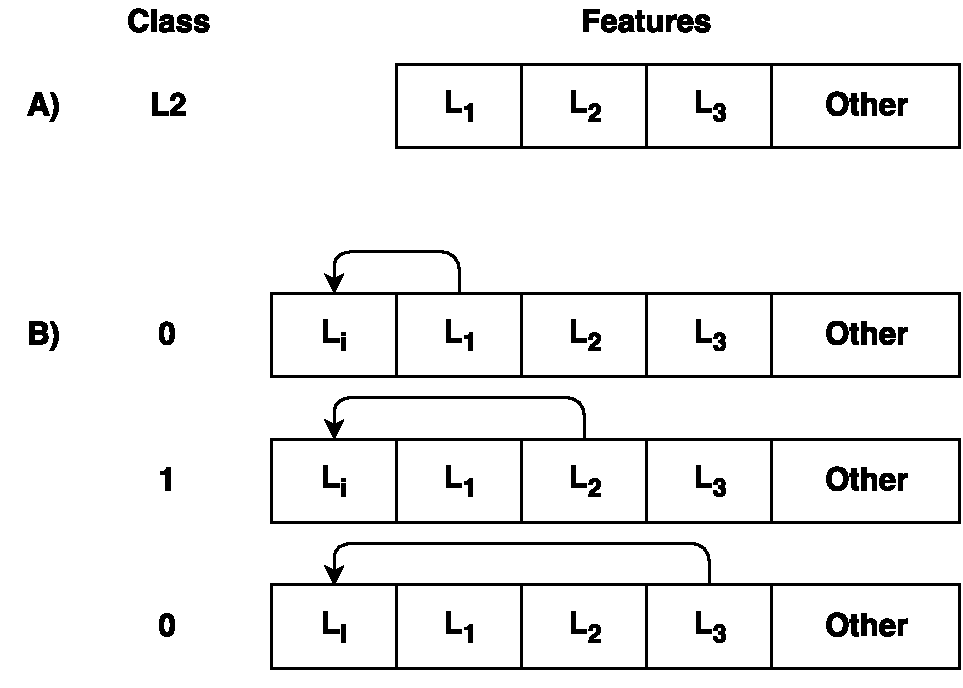
\includegraphics[scale=0.5]{multiclass.pdf}
 \end{figure}

  Using this approach we were able to create more general classifier, which works as a ranker of all considered languages.
  The final model was trained using RC-Rank algorithm which is internal algorithm of Seznam.cz suitable both for classification and ranking.
  It is based on gradient boosting over decision trees. The trees generated by algorithm are also oblivious, 
  which means that every split on the same level of tree is created on the same feature and value.
  This feature keeps the model safe from overfitting.

  \section{Training data}

  We used 3,456\footnote{We started by annotating over 4,000 pages.
  Unfortunately we didn't acquire all signals for all of them for technical reasons and thus
  we didn't make use of all the data in the end.} manually annotated 
  web pages randomly selected from database
  used by Seznam.cz's full-text search engine. Each URL was manually assigned
  to exactly one of 10 following language classes {\texttt{CS}, \texttt{DE},
  \texttt{EN}, \texttt{FR}, \texttt{PL}, \texttt{SK}, \texttt{UNKNOWN}, 
  \texttt{UNKNOWN\_CYRILLIC}, \texttt{UNKNOWN\_LATIN},
  \texttt{UNKNOWN\_OTHER}. 
  
  Web pages in the created set (represented by their
  URLs) were subsequently divided into two separate sets for training and
  testing. Our training set consisted of 2,410 web pages and our testing set
  contained the remaining 1,046 web pages. As soon as we realized that some
  language classes are obviously not sufficiently represented in our training
  data, we used the above-described trick ( constructing a single classifier for
  ten languages instead of ten different classifiers) to expand the data set as follows. 
  We looked at each example from the perspective of all ten languages. The 
  language-specific features remained the same for each ten clones of one example,
  but generic language features took values of the language whose perspective
  it was analyzed from  Thus, we generated nine false training instances and 
  one true in case of generic languages feature were properly set according to 
  language of manual  annotation. The final size of our datasets was
  24,100 and 10,460 samples for training and testing set respectively.


  \subsection{Features}
  Our classifier takes advantage of a total of 143 features (not including additional 96 mixed features) divided into four groups
  as follows: \textit{language-specific features}, \textit{generic language features}, \textit{non-language
  features} and \textit{mixed features}. In this section we briefly characterize each of these
  groups.

\subsubsection{Language-specific features}

  The classifier employs 110 language-specific features falling into 11 different  groups. Within each group a
  particular trait of a site is examined for each of 10 language classes separately. Selection of
  inspected language traits follows: 
  \begin{itemize}
    \item \textit{on-page language detection} - 
      %E.g. feature named \texttt{on\_page\_CS} 
      determines the probability of a web page being written in some particular
      %in the Czech 
      language based on analysis of all the text
      contained on the page with on-page detector based on (\cite{Rehurek:languageidentification} . 
      %Similarly \texttt{on\_page\_DE} determines the
      %probability for German language etc. 
      Besides the above-described analysis of whole text, the \textit{on-page 
      detector} is also used for analysing language of \textit{site-wide} text (\texttt{SWT}) and
    \textit{non-site-wide} text (\texttt{non-SWT}) separately. Site-wide text is a textual html element 
    present on all pages from a give site such as menus. The reason for that is that they might be 
    in different language than site-specific texts such as articles' bodies.
    \item \textit{backlink language prediction} - probabilities of the page being in a particular
      language based on language characteristics of other pages referencing to it 
      %(e.g.\texttt{backlink\_EN})
    \item \textit{language statistics aggregated for domains} - language statistics for the
      containing domains of different levels
    \item \textit{language specifications in} HTML - such as \texttt{<HTML lang=...>} or \texttt{<HTML
      meta http-equiv="Content-Language"  ...>}
    \item \text{selected language indicative tokens in URL} such as \texttt{cs} in:

    \texttt{http://www.europarl.europa.eu/news/}\underline{\texttt{cs}} 
    \item HTTP \textit{header field} \texttt{Content-language}
  \end{itemize}


 \subsubsection{Generic language features}
    For feature generation purposes, one can examine each web page from 10 different perspecitves -
    each corresponding to one particular language (i.e. a class). With generic language features, we
    take advantage of this fact by shifting from asking questions such as \textit{what is the probability that 
    this particular page is in the Czech language based on backlink statistics?} to questions 
    such as \textit{what is the probability that this page is in the language we are currently checking 
    based on backlink statistics?} Technically, this means simply
    that for each \textit{view} (i.e. particular language), we copy values of language-specific
    features for that language and use them as generic language features for the current view. Thus
    we end up with 11 generic language features (one for each trait group of language-specific
    features) such as \texttt{on\_page\_lang}, \texttt{backlink\_lang}, etc.
 \subsubsection{Non-language features}
    Not all used features are directly related to document language. Features in this group may help the
    classifier to first split the data space into distinct categories exhibiting different data patterns 
    to subsequently enhance the language detection itself.

    \begin{itemize}
      \item \textit{type of site} - probabilities of the site being an online marketplace, image gallery etc. We used
      our classififer trained to recognize such web sites.
      \item \textit{prices and currencies} - total numbers of matches of a set of regular
      expressions designed to detect prices in particular currencies (e.g. \texttt{\$35}) 
      \item \textit{text length} - defined as a number of tokens
      \item \textit{backlink count} - this feature was used in order to weight the influence of feature
      back-link language prediction.
    \end{itemize}

  \subsubsection{Mixed features}
    To make the job easier for the classifier, we also used mixed features which combine previously
    described features in various ways. Each of mixed features is either a sum or a product of a
    pair or a triplet of some selected features. 

    \section{Evaluation}
 For evaluation purpose we decided to compare proposed approach whith simple "majority vote"...CITACE.... as we were 
 not able to find other solutions dedicated for this particular task. We used 3000 training samples to create model. 
 The rest of labeled data - approximately 1900 examples - was used as testing dataset.
 
% \begin{table}[]
% \centering
% \caption{Evaluation results (in percents)}
% \label{evalres}
% \vspace{0.5cm}
% \begin{tabular}{l||c|c|c||c|c|c}
%       &
%     \multicolumn{3}{|c|}{\textbf{Majority vote}} &
%     \multicolumn{3}{|c}{\textbf{Our approach}} \\ \hline
%     \textbf{Lang.}    & \textbf{Prec.}  & \textbf{Rec.}   & \textbf{F1}    & \textbf{Prec.}  & \textbf{Rec.}   &  \textbf{F1}    \\ \hline
%     \textbf{Czech}    & 98.56  & 90.84  & 94.54 & 99.11  & 98.82  & 98.96  \\
%     \textbf{English}  & 86.67  & 97.76  & 91.88 & 96.78  & 99.21  & 97.98  \\
%     \textbf{Slovak}   & 97.10  & 80.72  & 88.16 & 98.80  & 98.80  & 98.80  \\
%     \textbf{German}   & 73.68  & 91.80  & 81.75 & 95.08  & 95.08  & 95.08  \\
%     \textbf{Polish}   & 81.82  & 94.74  & 87.80 & 100.00 & 100.00 & 100.00 \\
%     \textbf{French}   & 88.24  & 100.00 & 93.75 & 100.00 & 100.00 & 100.00 \\ \hline
%     \textbf{Latin}    & 85.71  & 61.94  & 71.91 & 96.50  & 89.03  & 92.62  \\
%     \textbf{Cyrillic} & 100.00 & 90.00  & 94.74 & 100.00 & 93.33  & 96.55  \\
%     \textbf{Other}    & 100.00 & 88.46  & 93.88 & 100.00 & 94.23  & 97.03  \\ \hline \hline
%     \textbf{W. sum.}  & 91.51  & 90.94  & 90.78 & 97.86  & 97.86  & 97.84  \\
% \end{tabular}
% \end{table}


\begin{table}[]
 \centering
 \caption{Evaluation results (in percents)}
 \label{evalres}
 \vspace{0.5cm}
 \begin{tabular}{l||c|c|c|}
       &
     \multicolumn{3}{|c}{\textbf{Majority vote}} \\ \hline
     \textbf{Lang.}    & \textbf{Prec.}  & \textbf{Rec.}   & \textbf{F1}  \\ \hline
     \textbf{Czech}    & 98.56  & 90.84  & 94.54 \\
     \textbf{English}  & 86.67  & 97.76  & 91.88 \\
     \textbf{Slovak}   & 97.10  & 80.72  & 88.16 \\
     \textbf{German}   & 73.68  & 91.80  & 81.75 \\
     \textbf{Polish}   & 81.82  & 94.74  & 87.80 \\
     \textbf{French}   & 88.24  & 100.00 & 93.75 \\ \hline
     \textbf{Latin}    & 85.71  & 61.94  & 71.91 \\
     \textbf{Cyrillic} & 100.00 & 90.00  & 94.74 \\
     \textbf{Other}    & 100.00 & 88.46  & 93.88 \\ \hline \hline
     \textbf{W. sum.}  & 91.51  & 90.94  & 90.78 \\
 \end{tabular}
 \end{table}


 \begin{table}[]
 \centering
 \caption{Evaluation results (in percents)}
 \label{evalres}
 \vspace{0.5cm}
 \begin{tabular}{l||c|c|c|}
       &
     \multicolumn{3}{|c}{\textbf{Our approach}} \\ \hline
     \textbf{Lang.}    & \textbf{Prec.}  & \textbf{Rec.}   & \textbf{F1} \\ \hline
     \textbf{Czech}    & 99.11  & 98.82  & 98.96  \\
     \textbf{English}  & 96.78  & 99.21  & 97.98  \\
     \textbf{Slovak}   & 98.80  & 98.80  & 98.80  \\
     \textbf{German}   & 95.08  & 95.08  & 95.08  \\
     \textbf{Polish}   & 100.00 & 100.00 & 100.00 \\
     \textbf{French}   & 100.00 & 100.00 & 100.00 \\ \hline
     \textbf{Latin}    & 96.50  & 89.03  & 92.62  \\
     \textbf{Cyrillic} & 100.00 & 93.33  & 96.55  \\
     \textbf{Other}    & 100.00 & 94.23  & 97.03  \\ \hline \hline
     \textbf{W. sum.}  & 97.86  & 97.86  & 97.84  \\
 \end{tabular}
 \end{table}

 In the result table we can observe that the simple majority vote F1 score was improved in average by 7\% (weighted average for all languages).
 The difference ranges from 10\% - 13\% for Slovak and German to smaller improvements above 4\% for Czech language.
 However, not all results for particular languages are so reliable as there were only few documents representing some of languages.
 This is obvious especially for Polish and French languages  where there were only 19, respectively 30 documents present 
 (another two smaller language groups were Cyrillic and Other).


 \section{Conclusions}
 Seznam.cz used to detect the major language of a website by hand crafted algorithm
 employing a decision tree with if conditions branches. Applying machine learning
 to this task brought Seznam.cz significant improvement in precision and recall in language detection.
 
 To make current algorhitm perform even better, we see an opportunity in web page type
 classifier. If it works with higher precision, it would be possible to set aside
 difficult web pages such as online marketplaces and the learning algorithm would be able to
 use different features.
 The above described approach towards major language detection has been implemented
 and is currently used in Seznam.cz to date.
\bibliographystyle{abbrv}
\bibliography{major_lang_paper}

\balancecolumns

% That's all folks!
\end{document}
